\documentclass[a4paper,12pt]{article} % This defines the style of your paper

\usepackage[top = 2.5cm, bottom = 2.5cm, left = 2.5cm, right = 2.5cm]{geometry} 

% Unfortunately, LaTeX has a hard time interpreting German Umlaute. The following two lines and packages should help. If it doesn't work for you please let me know.
\usepackage[T1]{fontenc}
\usepackage[utf8]{inputenc}
\usepackage{pifont}
% \usepackage{ctex}
\usepackage{amsthm, amsmath, amssymb, mathrsfs,mathtools}

% Defining a new theorem style without italics
\newtheoremstyle{nonitalic}% name
  {\topsep}% Space above
  {\topsep}% Space below
  {\upshape}% Body font
  {}% Indent amount
  {\bfseries}% Theorem head font
  {.}% Punctuation after theorem head
  {.5em}% Space after theorem head
  {}% Theorem head spec (can be left empty, meaning ‘normal’)
  
\theoremstyle{nonitalic}
% Define new 'solution' environment
\newtheorem{innercustomsol}{Solution}
\newenvironment{solution}[1]
  {\renewcommand\theinnercustomsol{#1}\innercustomsol}
  {\endinnercustomsol}

% Custom counter for the solutions
\newcounter{solutionctr}
\renewcommand{\thesolutionctr}{(\alph{solutionctr})}

% Environment for auto-numbering with custom format
\newenvironment{autosolution}
  {\stepcounter{solutionctr}\begin{solution}{\thesolutionctr}}
  {\end{solution}}


\newtheorem{problem}{Problem}
\usepackage{color}

% The following two packages - multirow and booktabs - are needed to create nice looking tables.
\usepackage{multirow} % Multirow is for tables with multiple rows within one cell.
\usepackage{booktabs} % For even nicer tables.

% As we usually want to include some plots (.pdf files) we need a package for that.
\usepackage{graphicx} 
\usepackage{subfigure}


% The default setting of LaTeX is to indent new paragraphs. This is useful for articles. But not really nice for homework problem sets. The following command sets the indent to 0.
\usepackage{setspace}
\setlength{\parindent}{0in}


% Package to place figures where you want them.
\usepackage{float}

% The fancyhdr package let's us create nice headers.
\usepackage{fancyhdr}

\usepackage{fancyvrb}

%Code environment 
\usepackage{listings} % Required for insertion of code
\usepackage{xcolor} % Required for custom colors

% Define colors for code listing
\definecolor{codegreen}{rgb}{0,0.6,0}
\definecolor{codegray}{rgb}{0.5,0.5,0.5}
\definecolor{codepurple}{rgb}{0.58,0,0.82}
\definecolor{backcolour}{rgb}{0.95,0.95,0.92}

% Code listing style named "mystyle"
\lstdefinestyle{mystyle}{
    backgroundcolor=\color{backcolour},   
    commentstyle=\color{codegreen},
    keywordstyle=\color{magenta},
    numberstyle=\tiny\color{codegray},
    stringstyle=\color{codepurple},
    basicstyle=\ttfamily\footnotesize, % Change to serif font
    breakatwhitespace=false,         
    breaklines=true,                 
    captionpos=b,                    
    keepspaces=true,                 
    numbers=left,                    
    numbersep=5pt,                  
    showspaces=false,                
    showstringspaces=false,
    showtabs=false,                  
    tabsize=2
}

\lstset{style=mystyle}

%%%%%%%%%%%%%%%%%%%%%%%%%%%%%%%%%%%%%%%%%%%%%%%%
% 3. Header (and Footer)
%%%%%%%%%%%%%%%%%%%%%%%%%%%%%%%%%%%%%%%%%%%%%%%%

% To make our document nice we want a header and number the pages in the footer.

\pagestyle{fancy} % With this command we can customize the header style.

\fancyhf{} % This makes sure we do not have other information in our header or footer.

\lhead{\footnotesize EI035 Econometrics I}% \lhead puts text in the top left corner. \footnotesize sets our font to a smaller size.

%\rhead works just like \lhead (you can also use \chead)
\rhead{\footnotesize Jingle Fu} %<---- Fill in your lastnames.

% Similar commands work for the footer (\lfoot, \cfoot and \rfoot).
% We want to put our page number in the center.
\cfoot{\footnotesize \thepage}
\IfFileExists{upquote.sty}{\usepackage{upquote}}{}
\begin{document}


\thispagestyle{empty} % This command disables the header on the first page. 

\begin{tabular}{p{15.5cm}} % This is a simple tabular environment to align your text nicely 
{\large \bf EI035 Econometrics I} \\
The Graduate Institute, Fall 2024, Marko Milkota\\
\hline % \hline produces horizontal lines.
\\
\end{tabular} % Our tabular environment ends here.

\vspace*{0.3cm} % Now we want to add some vertical space in between the line and our title.

\begin{center} % Everything within the center environment is centered.
	{\Large \bf PS2 Solutions} % <---- Don't forget to put in the right number
	\vspace{2mm}
	
        % YOUR NAMES GO HERE
	{\bf Jingle Fu} % <---- Fill in your names here!
		
\end{center}  

\vspace{0.4cm}
\setstretch{1.5}

\begin{autosolution}
    \

   \textbf{Step 1:} Write the pdf of observations $x_i | \theta$
   
   Since $x_i = \theta + u_i$, and we assume $u_i \sim \mathcal{N}(0, \sigma^2)$, then $x_i \sim \mathcal{N}(\theta, \sigma^2)$, and we have:
   \[
   p(x_i | \theta) = \frac{1}{\sqrt{2\pi\sigma^2}} \exp{\left\{-\frac{1}{2} \frac{(x_i - \theta)^2}{\sigma^2}\right\}}.
   \]

   \textbf{Step 2:} Define Likelihood Function

   We have assumed that observations in the sample are independent. Thus, 
   \[
   L_n(\theta) = \prod\limits_{i=1}^{n}p(x_i | \theta) = \left(\frac{1}{\sqrt{2\pi\sigma^2}}\right)^n \exp{\left\{-\frac{1}{2\sigma^2} \sum_{i=1}^{n} (x_i - \theta)^2\right\}}
   \]
   Log-linearize the function, and we define the log-likelihood function:
   \[
   \ell_{n}(\theta) = n\log{\left(\frac{1}{\sqrt{2\pi\sigma^2}}\right)} - \frac{1}{2\sigma^2} \sum_{i=1}^{n}(x_i - \theta)^2
   \]

   \textbf{Step 3:} Define the Likelihood Estimation problem and find the $\hat{\theta}$

   For maximum likelihood estimation, we need to solve the following problem:
   \[
       \hat{\theta}_{ML} = \arg\max\limits_{\theta \in \Theta}{L_n(\theta)} = \arg\max\limits_{\theta \in \Theta}{\ell_n(\theta)}
   \]
   So, we need to maximize:
   \[
   \ell_{n}(\theta) = n\log{\left(\frac{1}{\sqrt{2\pi\sigma^2}}\right)} - \frac{1}{2\sigma^2} \sum_{i=1}^{n}(x_i - \theta)^2
   \]
   Take the derivative of $\ell_n(\theta)$ with respect to $\theta$, and set it to zero for maximization,
   \begin{align*}
       \frac{\partial \ell_n(\theta)}{\partial \theta} &= \frac{1}{\sigma^2} \sum_{i=1}^{n}(x_i - \theta) \\
       &= \frac{1}{\sigma^2}(\sum_{i=1}^{n}x_i - n\theta) \\
       &= 0
   \end{align*}
   Thus, we have
   \[
   \hat{\theta}_{ML} = \frac{1}{n}\sum_{i=1}^{n}x_i
   \]
   
\end{autosolution}

\begin{autosolution}
    \ 

    \textbf{Step 1:} Find the likelihood function
    
    For $\mathcal{H}_0: \theta = \theta_0$, the likelihood function is:
    \[
    L_n(\theta_0) = \left(\frac{1}{\sqrt{2\pi\sigma^2}}\right)^n \exp{\left\{-\frac{1}{2\sigma^2} \sum_{i=1}^{n} (x_i - \theta_0)^2\right\}}
    \]
    For $\mathcal{H}_1: \theta \neq \theta_0$, the maximum likelihood estimator is $\hat{\theta}_{ML} = \frac{1}{n}\sum\limits_{i=1}^{n}x_i = \Bar{x}$. The likelihood function is:
    \[
    L_n(\theta_1) = \left(\frac{1}{\sqrt{2\pi\sigma^2}}\right)^n \exp{\left\{-\frac{1}{2\sigma^2} \sum_{i=1}^{n} (x_i - \Bar{x})^2\right\}}
    \]

    \textbf{Step 2:} Define the likelihood ratio test and $c_\alpha$

    The likelihood ratio and the test is firstly defined as follows(we'll simplify to another version later):
    \[
    \varphi_{LR}(x) = \mathbf{1}\left\{LR_n < c\right\}
    \]
    \begin{align*}
         LR_n &= \frac{L_n(\theta_1)}{L_n(\theta_0)} \\
              &= \exp{\left\{ \frac{1}{2\sigma^2}\left[\sum_{i=1}^{n} (x_i - \theta_0)^2 - \sum_{i=1}^{n} (x_i - \Bar{x})^2\right]\right\}}
    \end{align*}
    Denote 
    \[
    D = \sum\limits_{i=1}^{n} (x_i - \theta_0)^2 - \sum\limits_{i=1}^{n} (x_i - \Bar{x})^2
    \]
    Using the identity:
    \[
    \sum\limits_{i=1}^{n} (x_i - \theta_0)^2 = \sum\limits_{i=1}^{n} (x_i - \Bar{x} + \Bar{x} - \theta_0)^2 = \sum\limits_{i=1}^{n} (x_i - \Bar{x})^2 + n(\Bar{x} - \theta_0)^2
    \]
    Thus, 
    \begin{align*}
        D &= \sum\limits_{i=1}^{n} (x_i - \theta_0)^2 - \sum\limits_{i=1}^{n} (x_i - \Bar{x})^2 \\
          &= \sum\limits_{i=1}^{n} (x_i - \Bar{x})^2 + n(\Bar{x} - \theta_0)^2 - \sum\limits_{i=1}^{n} (x_i - \Bar{x})^2 \\
          &= n(\Bar{x} - \theta_0)^2 \\
          &= n(\hat{\theta} - \theta_0)^2
    \end{align*}
    So, the likelihood ratio $LR_n$ is:
    \[
    LR_n = \exp{\left\{\frac{n}{2\sigma^2} (\hat{\theta} - \theta_0)^2\right\}}
    \]
    Then, we simplify the expression and define the test statistic $T(x)$ as below:
    \[
    T(x) = 2\log{(LR_n)} = \frac{n}{\sigma^2}(\hat{\theta} - \theta_0)^2 = \frac{n}{\sigma^2}(x - \theta_0)^2
    \]
    And our LR test would be:
    \[
    \varphi_{LR}(x) = \mathbf{1}\left\{ T(x) = \frac{n}{\sigma^2}(x - \theta_0)^2 < c'\right\}
    \]
    where $c' = 2\log(c)$.
    To get a size $\alpha$ test, we find $c'$ so as to set the Type I error to $\alpha$, which is:
    \[
    \mathbb{P}\left[ T(x) \geq c' | \mathcal{H}_0\right] = \alpha
    \]
    we can denote that $c' = c_\alpha$.

    \textbf{Step 3:} Determine the distribution of $T(x)$ under $\mathcal{H}_0$ and find the value of $c_\alpha$

    Under $\mathcal{H}_0$, $\Bar{x} \sim \mathcal{N}(\theta_0, \frac{\sigma^2}{n})$, because:
    \begin{align*}
        \mathbb{E}[\Bar{x}] &= \mathbb{E}\left[\frac{1}{n}\sum\limits_{i=1}^{n}x_i\right] = \frac{1}{n}\sum\limits_{i=1}^{n}\mathbb{E}[x_i] = \frac{1}{n}\cdot n\theta_0 = \theta_0 \\
        \mathbb{V}[\Bar{x}] &= \mathbb{V}\left[ \frac{1}{n}\sum\limits_{i=1}^{n}x_i\right] = \frac{1}{n^2} \sum\limits_{i=1}^{n}\mathbb{V}[x_i] = \frac{1}{n}\cdot n\sigma^2 = \frac{\sigma^2}{n}
    \end{align*}
    Then, standardizing $\Bar{x}$, we'll have:
    \[
    Z = \frac{\Bar{x} - \theta_0}{\sqrt{\sigma^2/n}} \sim \mathcal{N}(0, 1)
    \]
    Using the hint, we know that
    \[
    Z^2 = \left(\frac{\Bar{x} - \theta_0}{\sqrt{\sigma^2/n}}\right)^2 = \frac{n}{\sigma^2}(\Bar{x} - \theta_0)^2 \sim \chi_{1}^{2}
    \]
    Therefore, under $\mathcal{H}_0$,
    \[
    T(x) = \frac{n}{\sigma^2}(x - \theta_0)^2 = Z^2 \sim \chi_{1}^2
    \]
    Given $\alpha=0.05$, 
    \[
    c_\alpha = \chi_{1, 0.95}^{2} \approx 3.84
    \]
    \textbf{Step 4:} Set the decision rule
    \begin{itemize}
        \item Reject $\mathcal{H}_0$: $T(x) > c_\alpha = 3.84$
        \item Do not reject  $\mathcal{H}_0$: $T(x) \leq c_\alpha = 3.84$
    \end{itemize}
\end{autosolution}

\begin{autosolution}
    \ 

    We have $\sigma^2=6$, $n=4$, $x_1=178$, $x_2=161$,$x_3=168$, $x_4=172$, $\theta_0=175$, so $\Bar{x}=169.75$.

    Put this data back into our $T(x)$ and LR test, we have:
    \[
    T(x) = \frac{n}{\sigma^2}(\Bar{x}-\theta_0)^2 = \frac{4}{6}(169.75-175)^2 = 18.735 > 3.84
    \]
    We reject $\mathcal{H}_0$.
\end{autosolution}

\begin{autosolution}
    \

\begin{lstlisting}[language=R]
rm(list = ls())
set.seed(2024)

theta_0 <- 175
sigma_squared <- 6
sigma <- sqrt(sigma_squared)
n <- 4
alpha <- 0.05
M <- 1000
T_values <- numeric(M)

for (m in 1:M) {
  x_m <- rnorm(n, mean = theta_0, sd = sigma)
  x_bar_m <- mean(x_m)
  T_m <- (n / sigma_squared) * (x_bar_m - theta_0)^2
  T_values[m] <- T_m
}

hist(T_values, breaks = 30, col = 'skyblue', border = 'black', freq = FALSE,
     main = 'Histogram of T(X) under H0', xlab = 'Test Statistic T(X)')
grid()

T_values_sorted <- sort(T_values)
c_alpha_index <- ceiling(M * (1 - alpha))
c_alpha <- T_values_sorted[c_alpha_index]

cat(sprintf('Numerical approximation of c_alpha: %.4f\n', c_alpha))

c_alpha_analytical <- qchisq(1 - alpha, df = 1)
cat(sprintf('Analytical c_alpha from chi-squared distribution: %.4f\n', c_alpha_analytical))

difference <- abs(c_alpha - c_alpha_analytical)
cat(sprintf('Difference between numerical and analytical c_alpha: %.4f\n', difference))
\end{lstlisting}
\ 

Numerical approximation of $c_\alpha$: 3.6266

Analytical$ c_\alpha$ from chi-squared distribution: 3.8415

\begin{figure}[!htbp]
    \centering
    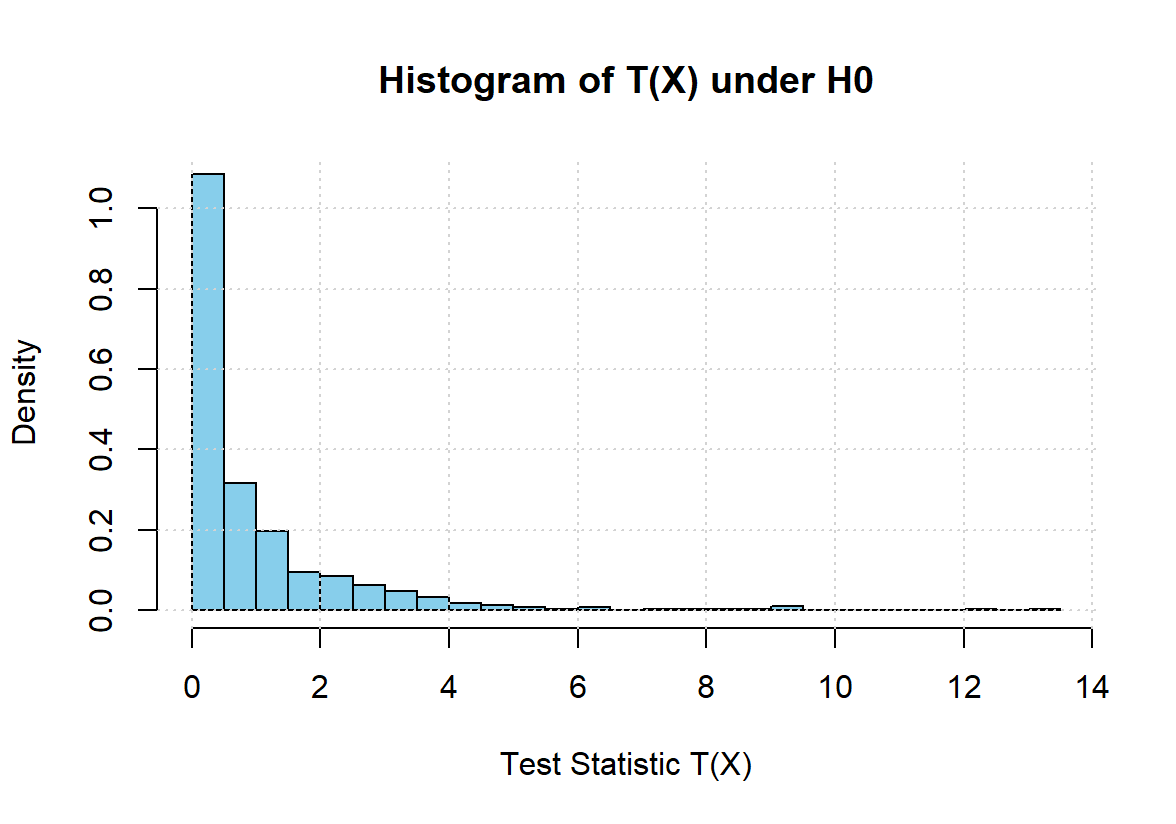
\includegraphics[width=1\linewidth]{R(d).png}
    \label{fig:R(d)}
\end{figure}

Difference between numerical and analytical $c_\alpha$: 0.2148, which is about 5.6\% of the analytical $c_\alpha$, so our approximation is not very close to the true value $c_\alpha$.

I expect the estimated approximation get closer to the real analytical value of $c_\alpha$ as $M$ is larger.

Since the $T(x)$ we get is 18.735 which is greatly larger than 3.84 and 3.62, which is our numerical result, the conclusion from previous exercise doesn't change, we still reject $\mathcal{H}_{0}$.
% \begin{lstlisting}[language=python]
% import numpy as np
% import matplotlib.pyplot as plt

% # Set the random seed for reproducibility
% np.random.seed(42)

% # Given parameters
% theta_0 = 175
% sigma_squared = 6
% sigma = np.sqrt(sigma_squared)
% n = 4
% alpha = 0.05
% M = 1000  # Number of simulations

% # Initialize an array to store the test statistics
% T_values = np.zeros(M)

% # Simulation loop
% for m in range(M):
%     # Draw a sample under H0: theta = theta_0
%     x_m = np.random.normal(theta_0, sigma, n)
%     # Compute the sample mean
%     x_bar_m = np.mean(x_m)
%     # Compute the test statistic T(x^m)
%     T_m = (n / sigma_squared) * (x_bar_m - theta_0) ** 2
%     # Store the test statistic
%     T_values[m] = T_m

% # Plot the histogram of T_values
% plt.figure(figsize=(10, 6))
% plt.hist(T_values, bins=30, color='skyblue', edgecolor='black', density=True)
% plt.title('Histogram of T(X) under H0')
% plt.xlabel('Test Statistic T(X)')
% plt.ylabel('Density')
% plt.grid(True)
% plt.show()

% # Sort the test statistics and find the critical value c_alpha
% T_values_sorted = np.sort(T_values)
% c_alpha_index = int(np.ceil(M * (1 - alpha))) - 1  # Adjust for zero-based index
% c_alpha = T_values_sorted[c_alpha_index]

% print(f'Numerical approximation of c_alpha: {c_alpha:.4f}')

% # Analytical critical value
% from scipy.stats import chi2
% c_alpha_analytical = chi2.ppf(1 - alpha, df=1)
% print(f'Analytical c_alpha from chi-squared distribution: {c_alpha_analytical:.4f}')

% # Compare the numerical and analytical critical values
% difference = abs(c_alpha - c_alpha_analytical)
% print(f'Difference between numerical and analytical c_alpha: {difference:.4f}')
% \end{lstlisting}
% \

% \begin{figure}[!htbp]
%     \centering
%     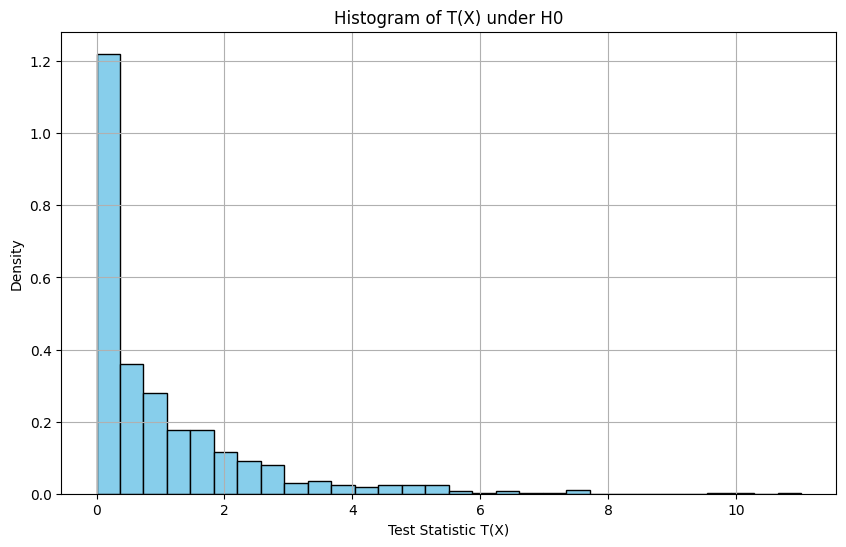
\includegraphics[width=\linewidth]{d.png}
%     \label{fig:(d)}
% \end{figure}
% Numerical approximation of $c_\alpha$: 3.9865

% Analytical $c_\alpha$ from chi-squared distribution: 3.8415

% Difference between numerical and analytical $c_\alpha$: 0.1450

\end{autosolution}


\begin{autosolution}
    \

    Based on our previous LR test, we have:
    \begin{align*}
        \varphi_{LR}(x) &= \mathbf{1}\left\{ T(x) = \frac{n}{\sigma^2}(x - \theta_0)^2 < c_\alpha\right\} \\
        &= \mathbf{1}\left\{ \frac{n}{\sigma^2}(\Bar{x} - \theta_0)^2 < c_\alpha\right\} \\
        &= \mathbf{1}\left\{(\Bar{x} - \theta_0)^2 < \frac{c_\alpha\sigma^2}{n}\right\} \\
        &= \mathbf{1}\left\{-\sqrt{\frac{c_\alpha\sigma^2}{n}} < (\Bar{x} - \theta_0) < \sqrt{\frac{c_\alpha\sigma^2}{n}}\right\} \\
        &= \mathbf{1}\left\{\Bar{x} -\sqrt{\frac{c_\alpha\sigma^2}{n}} < \theta_0 < \Bar{x} + \sqrt{\frac{c_\alpha\sigma^2}{n}}\right\}
    \end{align*}
    Thus, we can define $C(X)$ as:
    \[
    C(X) = \left[\Bar{x} -\sqrt{\frac{c_\alpha\sigma^2}{n}}, \Bar{x} +\sqrt{\frac{c_\alpha\sigma^2}{n}}  \right]
    \]
    Apply our previous data: $\sigma^2=6$, $n=4$, $x_1=178$, $x_2=161$,$x_3=168$, $x_4=172$, $\theta_0=175$, $\Bar{x}=169.75$, and $c_\alpha=3.84$, we have:
    \[
    C(X) = [169.75-2.4, 169.75+2.4] = [167.35, 172.15]
    \]
    $\theta_0=175$ is not in this interval.

    Because we rejected $\mathcal{H}_0: \theta=175$, it's consistent that 175 is not within the 95\% confidence interval.
\end{autosolution}

\begin{autosolution}
    \ 

\begin{lstlisting}[language=R]
rm(list = ls())
set.seed(2024)
M <- 1000 
alpha <- 0.05
n <- 4
sigma_squared <- 6
sigma <- sqrt(sigma_squared)
theta_values <- seq(160, 180, by = 0.1)
vc <- numeric(length(theta_values))

theta_true <- 175
x <- rnorm(n, mean = theta_true, sd = sigma)
x_bar <- mean(x)

for (i in seq_along(theta_values)) {
  theta_0 <- theta_values[i]
  
  T_values <- numeric(M)
  for (m in 1:M) {
    x_m <- rnorm(n, mean = theta_0, sd = sigma)
    x_bar_m <- mean(x_m)
    # Compute the test statistic T(x^m)
    T_m <- (n / sigma_squared) * (x_bar_m - theta_0)^2
    T_values[m] <- T_m
  }
  
  T_values_sorted <- sort(T_values)
  c_alpha_theta <- T_values_sorted[ceiling(M * (1 - alpha))]
  T_x_theta <- (n / sigma_squared) * (x_bar - theta_0)^2

  if (T_x_theta < c_alpha_theta) {
    vc[i] <- 1
  } else {
    vc[i] <- 0
  }
}

theta_in_Cx <- theta_values[vc == 1]
if (length(theta_in_Cx) > 0) {
  numerical_Cx <- c(min(theta_in_Cx), max(theta_in_Cx))
} else {
  cat("No values of theta_0 are included in the numerical confidence interval C(x).\n")
}

c_alpha <- qchisq(1 - alpha, df = 1)
margin <- sqrt((c_alpha * sigma_squared) / n)
analytical_Cx <- c(x_bar - margin, x_bar + margin)

plot(theta_values, vc, type = "p", col = "blue", pch = 16,
     main = "Numerical Confidence Interval C(x)",
     xlab = expression(theta[0] ~ "values"),
     ylab = expression(Indicator))
grid()
abline(v = analytical_Cx[1], col = 'red', lty = 2, lwd = 2)
abline(v = analytical_Cx[2], col = 'green', lty = 2, lwd = 2)

cat(sprintf("Numerical Confidence Interval C(x): [%.2f, %.2f]\n",
            numerical_Cx[1], numerical_Cx[2]))
cat(sprintf("Analytical Confidence Interval C(x): [%.2f, %.2f]\n",
            analytical_Cx[1], analytical_Cx[2]))
\end{lstlisting}

\begin{figure}[!htbp]
    \centering
    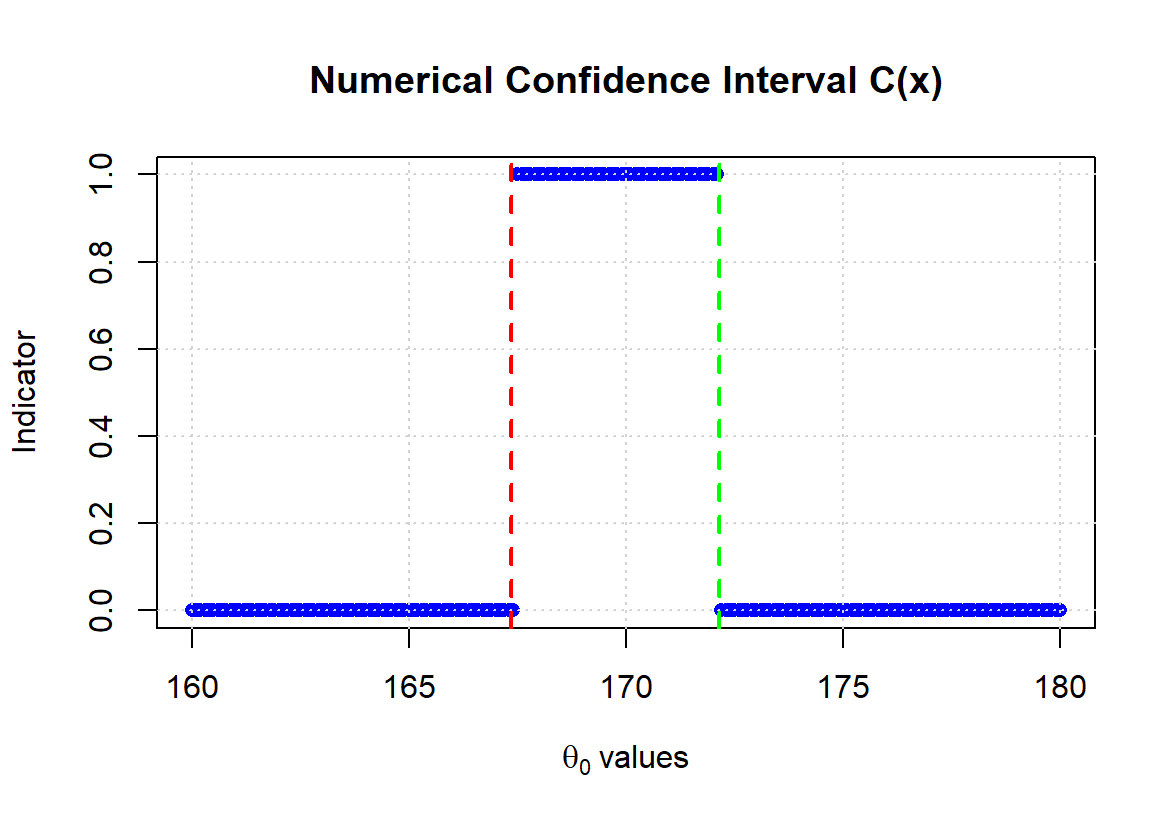
\includegraphics[width=1\linewidth]{R(f).png}
    \label{fig:R(f)}
\end{figure}
Numerical $C(x)$: [167.50, 172.10]

Analytical $C(x)$: [167.35, 172.15]

 The numerical confidence interval $C(x)$ aligns closely with the analytical interval, confirming our earlier findings that 175 is not included.


% \begin{lstlisting}[language=python]
% import numpy as np
% import matplotlib.pyplot as plt
% np.random.seed(2024)

% sigma_squared = 6
% sigma = np.sqrt(sigma_squared)
% n = 4
% alpha = 0.05
% M = 1000
% x = np.array([178, 161, 168, 172])
% x_bar = np.mean(x)

% T_values = np.arange(160, 180.1, 0.1)
% vc = []

% for theta_0 in T_values:
%     T_m = []
%     for _ in range(M):
%         x_m = np.random.normal(theta_0, sigma, n)
%         x_bar_m = np.mean(x_m)
%         T_m_value = (n / sigma_squared) * (x_bar_m - theta_0) ** 2
%         T_m.append(T_m_value)
%     c_alpha_theta = np.percentile(T_m, 95)
    
%     T_x_theta = (n / sigma_squared) * (x_bar - theta_0) ** 2
    
%     if T_x_theta < c_alpha_theta:
%         vc.append(1)
%     else:
%         vc.append(0)

% theta_in_Cx = T_values[np.array(vc) == 1]
% if len(theta_in_Cx) > 0:
%     numerical_Cx = [theta_in_Cx.min(), theta_in_Cx.max()]
%     print("Numerical Confidence Interval C(x): [{:.2f}, {:.2f}]".format(numerical_Cx[0], numerical_Cx[1]))
% else:
%     print("No values of theta_0 are included in the numerical confidence interval C(x).")

% plt.figure(figsize=(12, 6))
% plt.scatter(T_values, vc, c='blue', marker='o')
% plt.title('Numerical Confidence Interval C(x)')
% plt.xlabel('theta_0 values')
% plt.ylabel('Indicator (1 if theta_0 ∈ C(x), 0 otherwise)')
% plt.grid(True)
% plt.show()

% from scipy.stats import chi2

% c_alpha = chi2.ppf(1 - alpha, df=1)
% margin = np.sqrt((c_alpha * sigma_squared) / n)
% analytical_Cx = [x_bar - margin, x_bar + margin]

% print("Analytical Confidence Interval: [{:.2f}, {:.2f}]".format(analytical_Cx[0], analytical_Cx[1]))

% print("Comparison of Confidence Intervals:")
% print("Numerical C(x): [{:.2f}, {:.2f}]".format(numerical_Cx[0], numerical_Cx[1]))
% print("Analytical C(x): [{:.2f}, {:.2f}]".format(analytical_Cx[0], analytical_Cx[1]))
% \end{lstlisting}
% \ 

% \begin{figure}[!htbp]
%     \centering
%     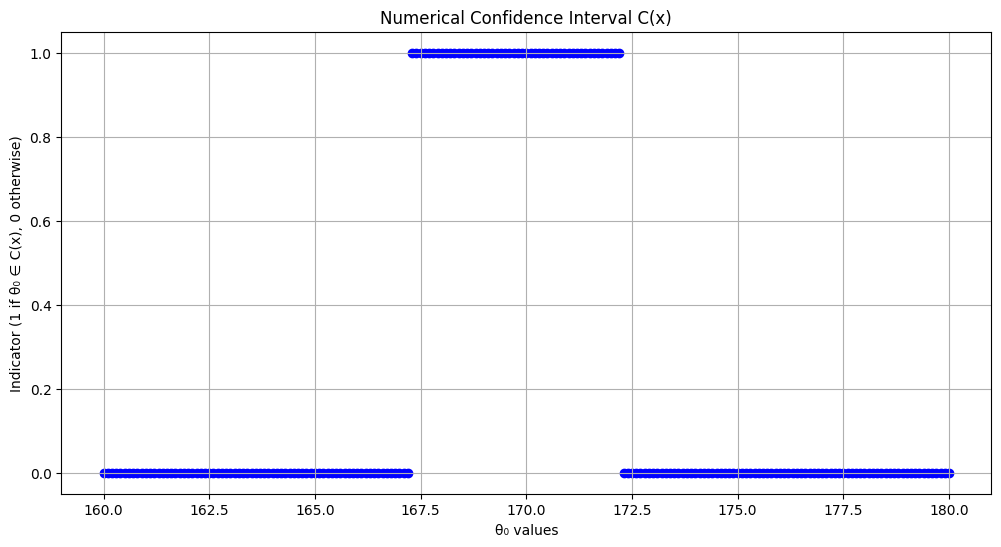
\includegraphics[width=1\linewidth]{(f).png}
%     \label{fig:(f)}
% \end{figure}

% Numerical C(x): [167.30, 172.20].

% Analytical C(x): [167.35, 172.15].

% The two results are very close to each other. 
    
\end{autosolution}

% \section*{Appendix}
% R code for problem (d):

% \

% % R code for problem (f):

\end{document}